\section{Διαδίκτυο των Πραγμάτων}
\label{sec:theory_iot}

Το διαδίκτυο των πραγμάτων περιγράφει το δίκτυο φυσικών αντικειμένων - "πραγμάτων" - που είναι ενσωματωμένα με αισθητήρες, λογισμικό και άλλες τεχνολογίες με σκοπό τη σύνδεση και την ανταλλαγή δεδομένων με άλλες συσκευές και συστήματα μέσω του διαδικτύου. Αυτές οι συσκευές μπορεί να είναι συνηθισμένα οικιακά αντικείμενα, ή και εξελιγμένα βιομηχανική εργαλεία. Με περισσότερες από 7 δισεκατομμύρια συνδεδεμένες συσκευές IoT σήμερα, οι ειδικοί αναμένουν ότι ο αριθμός αυτός θα αυξηθεί σε 10 δισεκατομμύρια έως το 2020 και 22 δισεεκατομμύρια έως το 2025.

Ένας ακόμη ορισμός για το IoT θα μπορούσε να είναι ο ακόλουθος:

\say{Ένα παγκόσμιο δίκτυο "πραγμάτων" που παρέχει μια ποικιλία πληροφοριών και επικοινωνιών, και αποτελείται από διασυνδεδεμένα δίκτυα χρησιμοποιώντας τυποποιημένα πρωτόκολλα επικοινωνίας.}

\subsection{Δομή του IoT}
\label{subsec:structure}

Οι φυσικές μονάδες (hardware unit) σε ένα σύστημα IoT αποτελείται από τις ακόλουθες κατηγορίες:

\begin{itemize}
	\item Αισθητήρες/ενεργοποιητές (Sensors/actuators)
	\item Μονάδες επεξεργασίας (Processing units)
	\item Μονάδες αποθήκευσης (Storage units)
	\item Μονάδες επικοινωνίας (Communication units)
\end{itemize}

Έχοντας προσδιορίσει της κατηγορίες του υλικού, ακολουθεί ο προσδιορισμός του λογισμικού, το ενδιάμεσο λογισμικό (middleware) και τα απαραίτητα πρωτόκολλα τα οποία παρέχουν τη δυνατότητα διασύνδεσης και επικοινωνίας με σκοπό τη συγκρότηση ενός πλήρως λειτουργικού IoT συστήματος \cite{bib:chebudie_2014}.

Σε αυτήν την ενότητα, παρουσιάζεται η αρχιτεκτονική του IoT. Στην ουσία, δεν υπάρχει μία συγκεκριμένη, καθώς διαφορετικές αρχιτεκτονικές έχουν προταθεί απο διαφορετικούς ερευνητές. Άρα θα παρουσιαστούν στη συνέχεια οι τρεις κυρίαρχες μορφές αρχιτεκτονικής, αυτές των τριών, τεσσάρων και πέντε επιπέδων (three-layer, four-layer, five-layer) \cite{bib:sethi_2017}.

\subsubsection{Αρχιτεκτονική 3 επιπέδων}
\label{subsubsec:3_layer}

Η αρχιτεκτονική 3 επιπέδων είναι η πιο βασική μορφή, και αποτελείται από τα επίπεδα αντίληψης, δικτύου και εφαρμογών, όπως φαίνεται και στο \autoref{fig:3_layer} \cite{bib:sethi_2017}.

\begin{figure}[!ht]
	\centering
	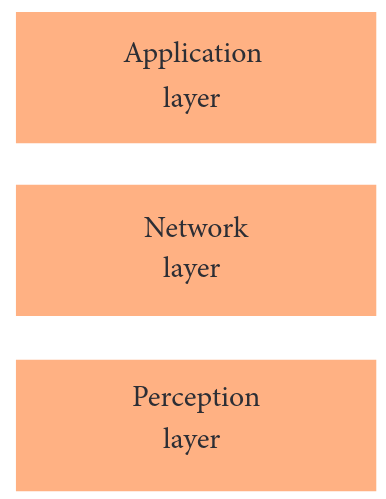
\includegraphics[width=0.3\textwidth]{./images/chapter3/3_layer.png}
	\caption{Αρχιτεκτονική IoT τριών επιπέδων.}
	\label{fig:3_layer}
\end{figure}

\textbf{\underline{Επίπεδο Αντίληψης}}

Το επίπεδο αντίληψης είναι το φυσικό επίπεδο, με αισθητήρες για την ανίχνευση και τη συλλογή πληροφοριών σχετικά με το περιβάλλον. Αυτό το επίπεδο ανιχνεύει κάποιες φυσικές παραμέτρους του περιβάλλοντος ή προσδιορίζει άλλα έξυπνα αντικείμενα στο περιβάλλον.

\textbf{\underline{Επίπεδο Δικτύου}}

Το επίπεδο δικτύου είναι υπεύθυνο για τη σύνδεση IoT στοιχείων με άλλα έξυπνα πράγματα, συσκευές δικτύου και διακομιστές. Η μετάδοση και η επεξεργασία δεδομένων των αισθητήρων πραγματοποιείται επίσης σε αυτό το επίπεδο.

\textbf{\underline{Επίπεδο Εφαρμογών}}

Το επίπεδο εφαρμογών είναι υπεύθυνο για την παροχή υπηρεσιών συγκεκριμένης εφαρμογής (application specific services) στον χρήστη. Οι σχεδιαστικές του παράμετροι διέπουν τις διάφορες εφαρμογές (έξυπνο σπίτι, έξυπνη πόλη, υγειονομική περίθαλψη κ.α.) στις οποίες μπορεί να αναπτυχθεί το IoT.

\subsubsection{Αρχιτεκτονική 4 επιπέδων}
\label{subsubsec:4_layer}

Αυτή η μορφή αρχιτεκτονικής είναι ελαφρώς διαφορετική από αυτήν των τριών επιπέδων. Αποτελείται από τα επίπεδα εφαρμογών, επεξεργασίας δεδομένων, δικτύου και αντίληψης/αισθητήρων, όπως φαίνεται και στο \autoref{fig:4_layer} \cite{bib:kumar_2018}.

\begin{figure}[!ht]
	\centering
	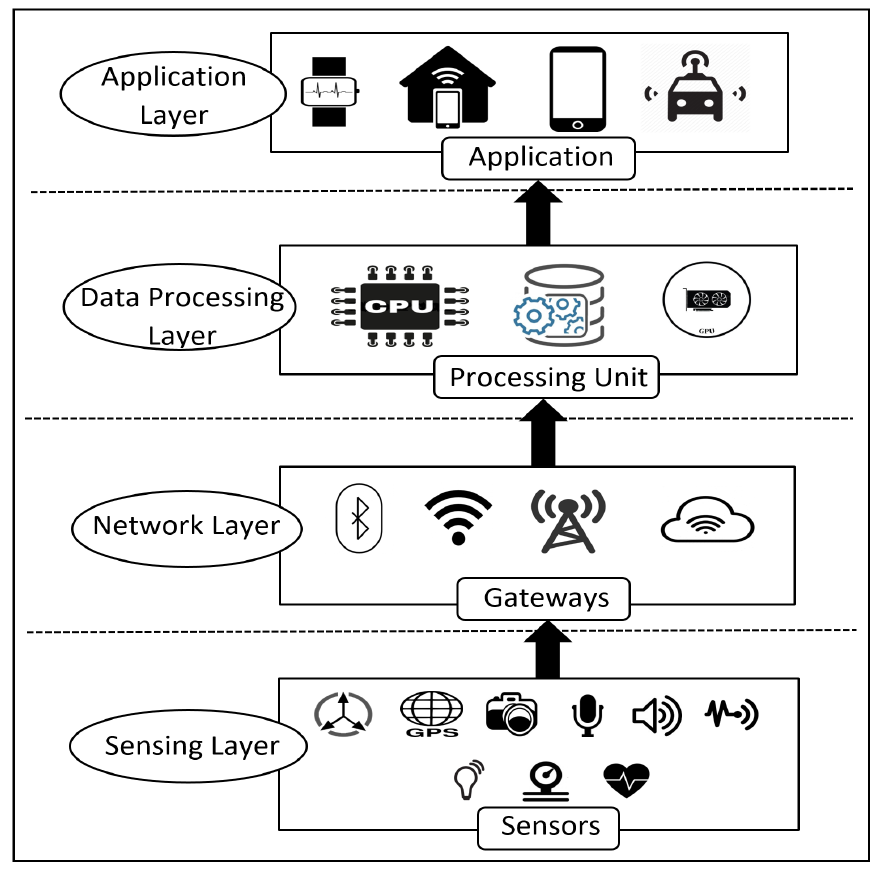
\includegraphics[width=0.5\textwidth]{./images/chapter3/4_layer.png}
	\caption{Αρχιτεκτονική IoT τεσσάρων επιπέδων.}
	\label{fig:4_layer}
\end{figure}

\textbf{\underline{Επίπεδο Αντίληψης/Αισθητήρων}}

Ο βασικός ρόλος του επιπέδου αυτού είναι να ανιχνεύσει οποιαδήποτε φαινόμενα στο περιβάλλον των συσκευών και να λάβει δεδομένα από τον πραγματικό κόσμο. Οι αισθητήρες σε ένα δίκτυο μπορεί να είναι διαφόρων τύπων και το επίπεδο αντίληψης πρέπει να είναι σε θέση να τους διαφοροποιεί και να προσαρμόζει τις διαφορετικές μεθόδους λειτουργίας τους. 

\textbf{\underline{Επίπεδο Δικτύου}}

Το επίπεδο αυτό δρα ως κανάλι επικοινωνίας για τη μεταφορά δεδομένων, τα οποία συλλέχτηκαν στο επίπεδο αίσθησης, σε άλλες συνδεδεμένες συσκευές. Στις IoT συσκευές το επίπεδο δικτύου υλοποιείται με τη χρήση ποικίλων τεχνολογιών επικοινωνίας, όπως Wi-Fi, Bluetooth, Zegbee, Z-Wave, LoRa κ.α.

\textbf{\underline{Επίπεδο Επεξεργασίας Δεδομένων}}

Το επίπεδο επεξεργασίας δεδομένων αποτελείται από την κεντρική μονάδα επεξεργασίας των IoT συσκευών. Λαμβάνει τα δεδομένα από το επίπεδο αίσθησης, και τα αναλύει με σκοπό να πάρει αποφάσεις βάση του αποτελέσματος. Σε κάποιες IoT συσκευές, το επίπεδο αυτό αποθηκεύει το αποτέλεσμα προηγούμενων αναλύσεων με σκοπό τη βελτίωση της εμπειρίας χρήστη. Τέλος, μπορεί να μοιραστεί τα αποτελέσματα των αναλύσεων με άλλες συνδεδεμένες συσκευές μέσω του επιπέδου δικτύου.

\textbf{\underline{Επίπεδο Εφαρμογών}}

Το επίπεδο εφαρμογών ορίζει όλες τις εφαρμογές στις οποίες αναπτύσσεται το IoT και παρέχει τη διεπαφή μεταξύ των IoT συσκευών και του δικτύου. Αυτό το επίπεδο υλοποιεί και παρουσιάζει τα αποτελέσματα του επιπέδου επεξεργασίας δεδομένων ώστε να εκτελέσει διάφορες λειτουργίες των IoT συσκευών.

\subsubsection{Αρχιτεκτονική 5 επιπέδων}
\label{subsubsec:5_layer}

Επιπρόσθετα από τα επίπεδα αντίληψης, δικτύου και εφαρμογών της αρχιτεκτονικής τριών επιπέδων, η αρχιτεκτονική πέντε επιπέδων περιλαμβάνει τα επίπεδα επεξεργασίας και επιχειρήσεων, όπως φαίνεται και στο \autoref{fig:5_layer} \cite{bib:sethi_2017}. Ο ρόλος των επιπέδων αντίληψης και εφαρμογών σε αυτό το μοντέλο είναι ο ίδιος με την αρχιτεκτονική με τρία επίπεδα.

\begin{figure}[!ht]
	\centering
	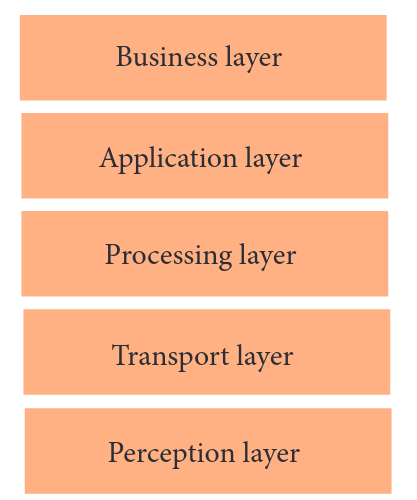
\includegraphics[width=0.3\textwidth]{./images/chapter3/5_layer.png}
	\caption{Αρχιτεκτονική IoT πέντε επιπέδων.}
	\label{fig:5_layer}
\end{figure}

\textbf{\underline{Επίπεδο Μεταφοράς}}

Το επίπεδο μεταφοράς παίρνει τη θέση του επιπέδου δικτύου, και μεταφέρει δεδομένα αισθητήρων από προς το επίπεδο αντίληψης και το επίπεδο επεξεργασίας. Για τον σκοπό αυτό, χρησιμοποιούνται δίκτυα όπως ασύρματα, 3/4G, τοπικά (LAN), Bluetooth, RFID, NFC κ.α.

\textbf{\underline{Επίπεδο Επεξεργασίας}}

Το επίπεδο επεξεργασίας είναι επίσης γνωστό ως επίπεδο middleware και είναι υπεύθυνο για την αποθήκευση, ανάλυση και επεξεργασία των τεράστιων όγκων δεδομένων που προέρχονται από το επίπεδο μεταφοράς. Χρησιμοποιώντας τεχνολογίες όπως βάσεις δεδομένων, υπολογιστικό νέφος και μονάδες επεξεργασίας μεγάλων δεδομένων, μπορεί να διαχειριστεί και να προσφέρει ένα ποικίλο σύνολο υπηρεσιών στα χαμηλότερα επίπεδα.

\textbf{\underline{Επίπεδο Επιχείρησης}}

Το επίπεδο επιχείρησης διαχειρίζεται ολόκληρο το IoT σύστημα, συμπεριλαμβανομένων των εφαρμογών του, των επιχειρηματικών και κερδοφόρων μοντέλων του και της ιδιωτικότητας των χρηστών (user privacy).